\section{Propuesta}

\subsection{Descripción}

\subsection{Herramientas de desarrollo elegidas}

\subsection{Ciclo de vida/Metodología}
En esta sección hableremos de la métodología empleada, que en este caso hemos decidido usar la famosa metodología ágil scrum. \\

En este caso debido a la fluctuación temporal hemos decicido hacer sprints largos de un mes. Con esto tratamos de conseguir obtener un prototipo con cambios considerables a lo largo de cada sprint.


\subsection{Iteración 0}

Hablando con las asociaciones nos hemos dado cuenta de que los intercambios de acogidas no son una buena idea por lo que se ha descartado. \\
\subsubsection{Product Backlog}
Prioridades hechas con MoSCoW (tema 4 MDA)
\begin{table}[H]
    \centering
    \begin{tabular}{|c |p{8cm}|c |c|} \hline 
         \multirow[c]{3}{*}{Usuario}&  \textbf{Tarea}&  \textbf{Coste}& \textbf{Prio.}\\  \cline{2-4}%Prio. es de prioridad 
         &  Acceder a la aplicación&  5& M\\ \cline{2-4} 
         &  Cerrar sesión&  1& M\\ \hline 
    \end{tabular}
    \caption{Product backlog de usuarios}
    \label{tab:pb_usuarios}
\end{table}

\begin{table}[H]
    \centering
    \begin{tabular}{|c |p{8cm}|c |c|} \hline 
         \multirow[c]{23}{*}{Asociación}&  \textbf{Tarea}&  \textbf{Coste}& \textbf{Prio.}\\  \cline{2-4}
         
         &  Registrame en la aplicación como asociación&  5& M\\ \cline{2-4} 
         &  Poner animales en adopción&  8& M\\ \cline{2-4} 
         &  Anular poner animales en adopción&  3& M\\ \cline{2-4} 
         &  Ver solucitudes adopción&  5& M\\ \cline{2-4}
         &  Aceptar solucitudes adopción&  3& M\\ \cline{2-4}
         &  Rechazar solucitudes adopción&  3& M\\ \cline{2-4}
         
         
         &  Poner animales en acogida&  3& M\\ \cline{2-4}
         &  Anular poner animales en acogida&  3& M\\ \cline{2-4} 
         &  Ver solucitudes acogida&  3& M\\ \cline{2-4}
        
         &  Ver que usuarios tienen a sus animales en acogida&  5& M\\ \cline{2-4}
         &  Buscar usuarios que estén como casa de acogida&  5& M\\ \cline{2-4}
         &  Solicitar acogida a particular &  5& M\\ \cline{2-4}
         
         
         &  Decidir si desean ser voluntarios o no&  3& M\\ \cline{2-4}
         &  Ver solicitudes voluntariado propias&  3& M\\ \cline{2-4}
         &  Aceptar solucitudes voluntariado&  3& M\\ \cline{2-4}
         &  Rechazar solucitudes voluntariado&  3& M\\ \cline{2-4}
         
         &  Mandar contrato adopción firmado al adoptante&  8& S\\ \cline{2-4}
         
         &  Elegir si poner a sus animales como apadrinables o no &  5& S\\ \cline{2-4}
         &  Rechazar solucitudes voluntariado&  3& M\\ \cline{2-4}
         
         &  Modificar su descripción para que los usuarios vean a que se dedican & 5 & M \\ \hline

         
         
        
    \end{tabular}
    \caption{Product backlog de Asociaciones}
    \label{tab:pb_asociaciones}
\end{table}


\begin{table}[H]
    \centering
    \begin{tabular}{|c |p{8cm}|c |c|} \hline 
         \multirow[c]{14}{*}{Particular}&  \textbf{Tarea}&  \textbf{Coste}& \textbf{Prio.}\\  \cline{2-4}
         &  Registrame en la aplicación como particular&  5& M\\ \cline{2-4} 
         

         &  Solicitar adopciones&  3& M\\ \cline{2-4}
         &  Ver adopciones pendientes&  3& S\\ \cline{2-4}
         
         &  Solicitar acogidas&  3& M\\ \cline{2-4} 
         &  Ver acogidas pendientes&  3& M\\ \cline{2-4}
       
         &  Ponerse como casa de acogida&  3& S\\ \cline{2-4}
         
         &  Cumplimentar el formulario de solicitud de adopciones/acogidas &  5& S\\ \cline{2-4}
		 &  Firmar contrato de adopción electrónicamente&  8& S\\ \cline{2-4}
		 
		 
         &  Solicitar voluntariados&  3& M\\ \cline{2-4} 
         &  Ver voluntariados pendientes&  3& M\\ \cline{2-4}
         &  Ver historial voluntariados&  5& C\\ \cline{2-4}
         
         
         & Apadrinar a un animal&  5& S\\ \hline
         
         
         
    \end{tabular}
    \caption{Product backlog de Particulares}
    \label{tab:pb_particulares}
\end{table}

\begin{table}[H]
    \centering
    \begin{tabular}{|c |p{8cm}|c |c|} \hline 
         \multirow[c]{17}{2cm}{Asociación y Particular}&  \textbf{Tarea}&  \textbf{Coste}& \textbf{Prio.}\\  \cline{2-4}

         &  Ver su perfil &  5& M\\ \cline{2-4}
         &  Modificar su perfil &  5& M\\ \cline{2-4}
         &  Eliminar su perfil &  3& M\\ \cline{2-4}
         
         &  Aceptar solucitudes acogida&  3& M\\ \cline{2-4}
         &  Rechazar solucitudes acogida&  3& M\\ \cline{2-4}
         
         &  Ver historial de adopciones &  5& M\\ \cline{2-4}
         &  Ver historial de acogidas &  5& M\\ \cline{2-4}
         &  Eliminar sus publicaciones &  3& M\\ \cline{2-4}
         
         & Poner aviso de animal perdido encontrado & 5 & M \\ \cline{2-4}
         & Ver lista de animales perdidos & 5 & M \\ \cline{2-4}

         &  Reportar un perfil &  1& M\\ \cline{2-4}
         &  Reportar una publicación &  1& M\\ \cline{2-4}
         
         &  Realizar el seguimiento de adoción de la mascota adoptada&  8& C\\ \cline{2-4}
         
         &  Chatear con otros usuarios a raiz de una adopción/acogida/voluntariado &  8& M\\ \hline

         
         
    \end{tabular}
    \caption{Product backlog de Particulares y Asociaciones}
    \label{tab:pb_aso_particular}
\end{table}

\begin{table}[H]
    \centering
    \begin{tabular}{|c |p{8cm}|c |c|} \hline 
         \multirow[c]{4}{2cm}{Us. Básico y Particular}&  \textbf{Tarea}&  \textbf{Coste}& \textbf{Prio.}\\  \cline{2-4}
         
		 &  Buscar anuncios en una zona concreta&  5& S\\ \cline{2-4}		
         &  Ver peticiones de adopción&  8& M\\ \hline

         
         
    \end{tabular}
    \caption{Product backlog de Us. Básico y Particulares}
    \label{tab:pb_part_usBasico}
\end{table}

\begin{table}[H]
    \centering
    \begin{tabular}{|c|p{8cm}|c|c|} \hline 
         \multirow[c]{4}{*}{Administrador}&  \textbf{Tarea}&  \textbf{Coste}& \textbf{Prio.}\\  \cline{2-4}
         &  Crear usuarios &  5& M\\ \cline{2-4}
         &  Modificar usuarios &  5& M\\ \cline{2-4}
         &  Eliminar usuarios &  3& M\\ \hline

         
         
    \end{tabular}
    \caption{Product backlog de Administradores}
    \label{tab:pb_administradores}
\end{table}

\begin{table}[H]
    \centering
    \begin{tabular}{|c|p{8cm}|c|c|} \hline 
         \multirow[c]{7}{*}{Moderador}&  \textbf{Tarea}&  \textbf{Coste}& \textbf{Prio.}\\  \cline{2-4}
         &  Ver publicaciones reportadas &  5& M\\ \cline{2-4}
         &  Eliminar publicaciones reportadas &  3& M\\ \cline{2-4}

         &  Ver usuarios reportados &  5& M\\ \cline{2-4}
         &  Banear usuarios reportados &  3& M\\ \cline{2-4}
         
         &  Ver lista de asociaciones recién registradas &  5& M\\ \cline{2-4}
         &  Validar las asociaciones recién registradas& 5 & M\\ \hline

         
         
    \end{tabular}
    \caption{Product backlog de Moderadores}
    \label{tab:pb_moderadores}
\end{table}

Una vez creadas todas las historias de usuario procedemos a su planificación y asignación en los diferentes sprints, la idea es hacer un scrum con sprints de un mes. A continucación se muestran las tareas asignadas a cada sprint: \\ \\

Sprint 1 \\ 
\begin{figure}[H]
	\centering
	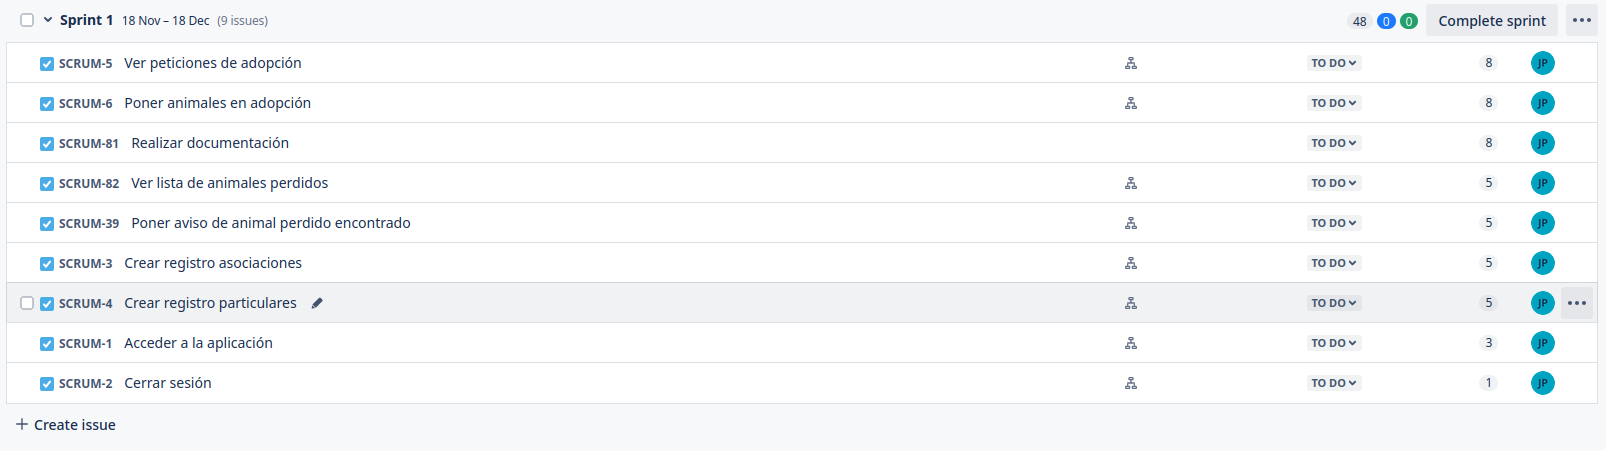
\includegraphics[width=1\linewidth]{screenshot001}
	\caption{Planificación del primer sprint}
	\label{fig:sprint1}
\end{figure}


Sprint 2 \\
\begin{figure}[H]
	\centering
	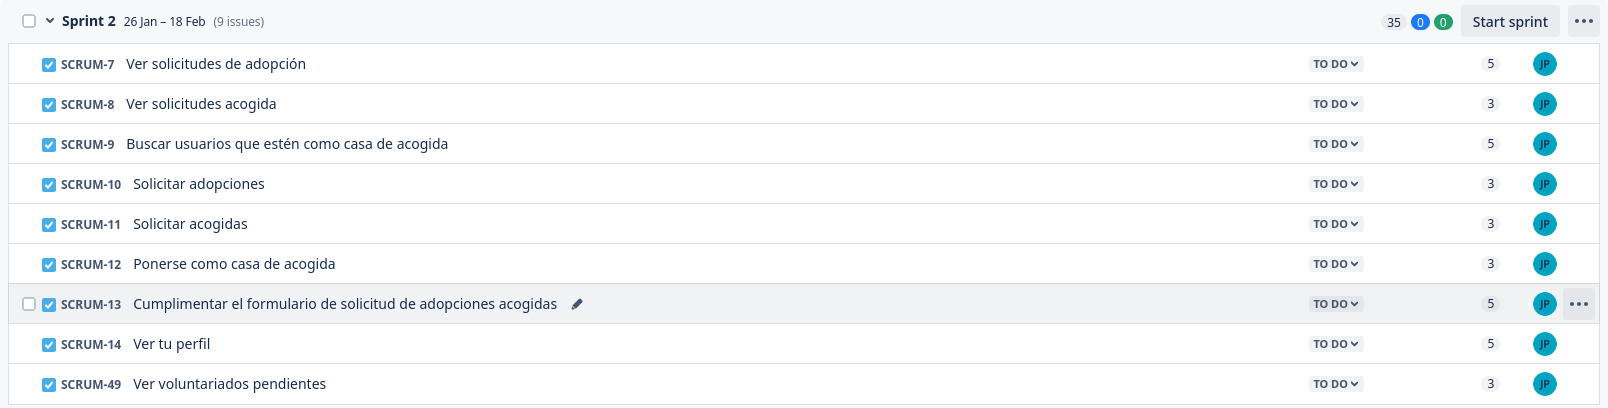
\includegraphics[width=1\linewidth]{screenshot002}
	\caption{Planificación del segundo sprint}
	\label{fig:sprint2}
\end{figure} 


Sprint 3 \\ 
\begin{figure}[H]
	\centering
	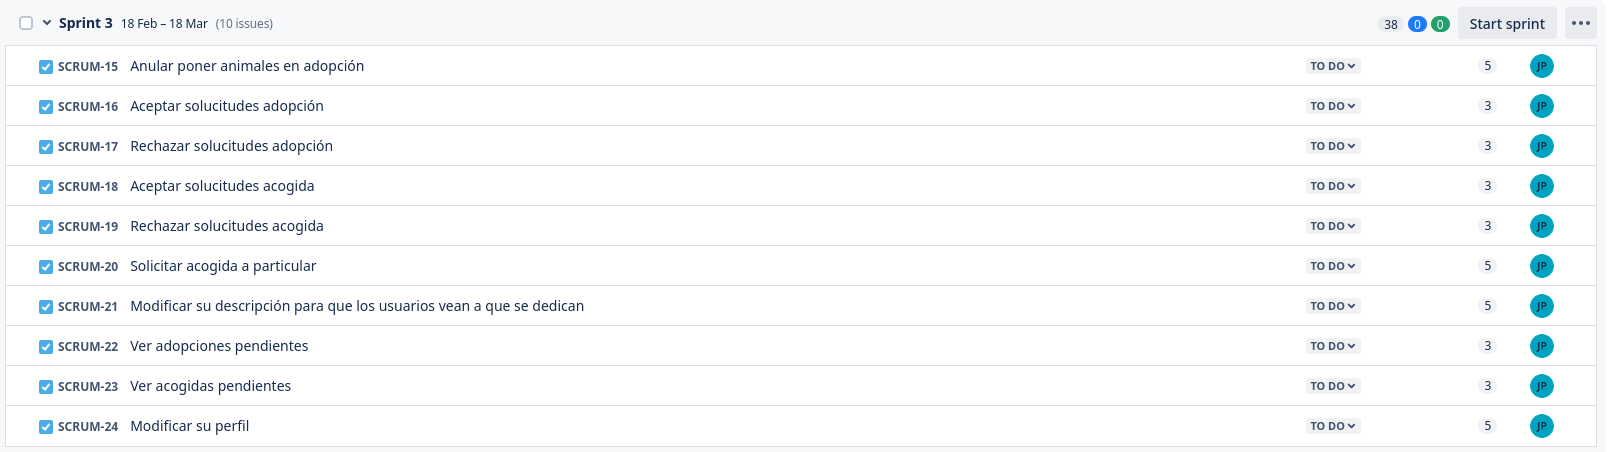
\includegraphics[width=1\linewidth]{sprint3}
	\caption{Planificación del tercer sprint}
	\label{fig:sprint3}
\end{figure}

Sprint 4 \\
\begin{figure}[H]
	\centering
	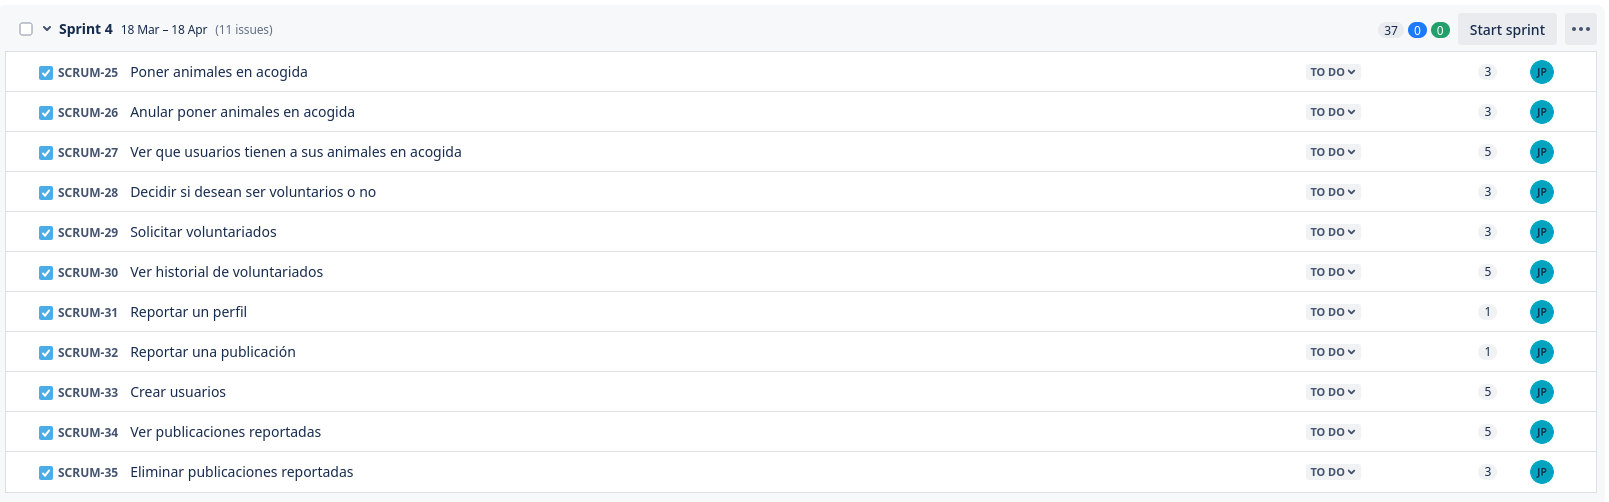
\includegraphics[width=1\linewidth]{sprint4}
	\caption{Planificación del cuarto sprint}
	\label{fig:sprint4}
\end{figure}

Sprint 5 \\ 
\begin{figure}[H]
	\centering
	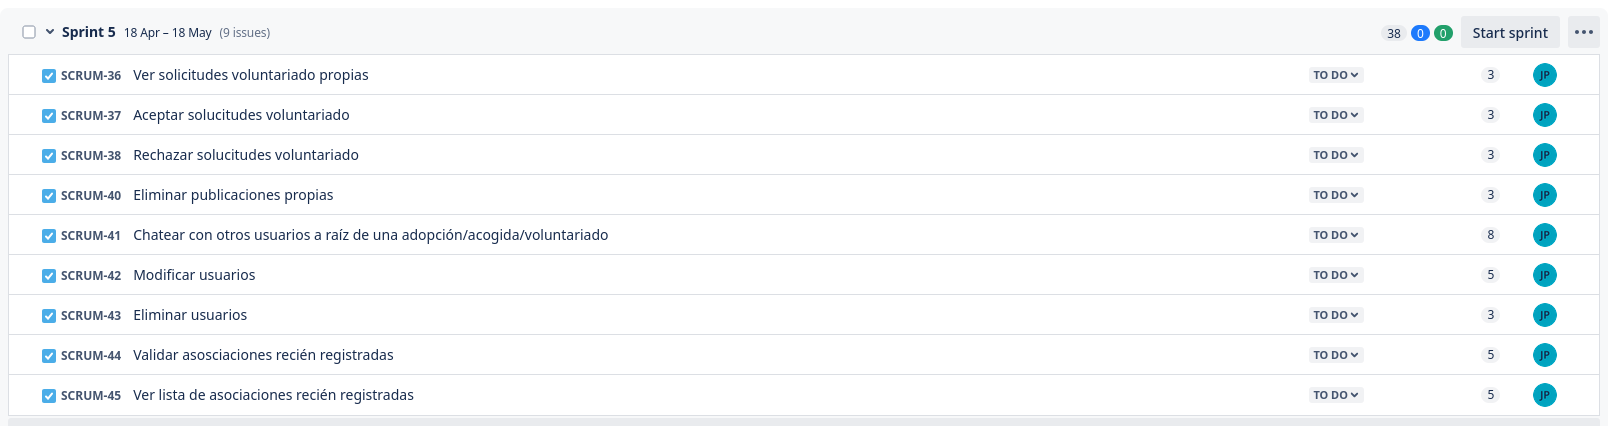
\includegraphics[width=1\linewidth]{sprint5}
	\caption{Planificación del quinto sprint}
	\label{fig:sprint5}
\end{figure}

Product backlog restante \\
\begin{figure}[H]
	\centering
	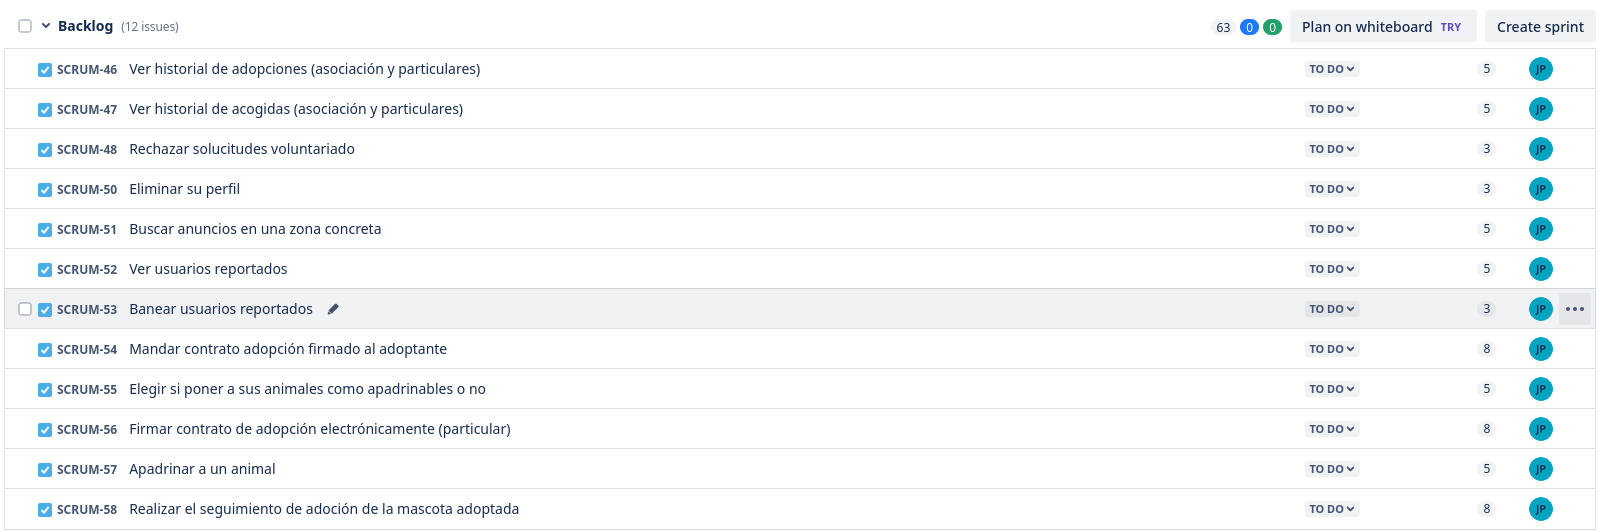
\includegraphics[width=1\linewidth]{pb}
	\caption{Tareas a hacer en siguientes sprints}
	\label{fig:pb_restante}
\end{figure}





\subsection{Iteración 1}

\large{\textbf{Especificación de tareas}} \\


\begin{tabular}{|c|p{9.5cm}|p{1cm}|}
	\hline
	\multicolumn{3}{|c|}{\textbf{HU.1 - Ver animales en adopción}} \\
	\hline
	\textbf{Id} & \textbf{Título de la tarea de desarrollo} & \textbf{Est. (días)} \\
	\hline
	1.1 & Realizar bocetos & 0.5 \\ \hline
	1.2 &  Implementar interfaz para ver las adopciones disponible & 2 \\ \hline
	1.3 &  Implementar la lógica de obtención de animales en adopción & 1 \\ \hline
	\multicolumn{3}{|c|}{\textbf{Pruebas de aceptación}} \\ \hline
	1 & \multicolumn{2}{|l|}{Mostrar mensaje en caso de que no haya animales} \\ \hline
	2 & \multicolumn{2}{|l|}{Mostrar lista de todos los animales} \\ \hline
	3 & \multicolumn{2}{|l|}{Que los filtros funcionen correctamente} \\ \hline
	
\end{tabular} \\ \\

\label{sec:hu1}

\begin{tabular}{|c|p{9.5cm}|p{1cm}|}
	\hline
	\multicolumn{3}{|c|}{\textbf{HU.2 - Poner animales en adopción}} \\
	\hline
	\textbf{Id} & \textbf{Título de la tarea de desarrollo} & \textbf{Est. (días)} \\ %Est. es estimación
	\hline
	2.1 & Realizar bocetos & 0.5 \\ \hline
	2.2 &  Implementar interfaz para añadir animales en adopción & 2 \\ \hline
	2.3 &  Insertar datos de animales en la bd & 2 \\ \hline 
	\multicolumn{3}{|c|}{\textbf{Pruebas de aceptación}} \\ \hline
	1 & \multicolumn{2}{|l|}{Mostrar avisos en caso de error en el fomulario} \\ \hline
	2 & \multicolumn{2}{|l|}{Previsualizar imágenes asociadas al animal} \\ \hline
	3 & \multicolumn{2}{|l|}{Poder eliminar imágenes concretas antes subirlas al servidor} \\ \hline
\end{tabular} \\ \\


\begin{tabular}{|c|p{9.5cm}|p{1cm}|}
	\hline
	\multicolumn{3}{|c|}{\textbf{HUT.1 - Realizar documentación}} \\
	\hline
	\textbf{Id} & \textbf{Título de la tarea de desarrollo} & \textbf{Est. (días)} \\
	\hline
	1.1 & Realizar documentación para cada tarea & 3 \\ \hline
	1.2 &  Añadir tareas a las historias de usuario & 0.5 \\ \hline
\end{tabular} \\ \\

\begin{tabular}{|c|p{9.5cm}|p{1cm}|}
	\hline
	\multicolumn{3}{|c|}{\textbf{HUT.2 - Aprender las tecnologías a utilizar}} \\
	\hline
	\textbf{Id} & \textbf{Título de la tarea de desarrollo} & \textbf{Est. (días)} \\
	\hline
	2.1 & Buscar documentación sobre sequelize & 1.5 \\ \hline
	2.2 & Buscar documentación sobre Ionic & 1.5 \\ \hline
\end{tabular} \\ \\


Una vez planificadas todas las historias de usuario del sprint empezaremos a realizarlas preferentemente en el orden designado. \\ \\

\Large{\textbf{HU.1 - Ver animales en adopción}} \\

En esta historia nos encargamos de la visualización de los distintos animales de adopción y su filtrado en función a unos parámetros clave, en este caso se han elegido la edad, la especie, y la localización. \\

Además por otra parte cabe destacar que esta será la página principal para los usuarios particulares. \\ 

\textbf{Bocetos}

Lo primero es crear los bocetos de la página para ello hemos hecho uso de la herramienta draw.io la cual permite realizar bocetos simples en poco tiempo.

\begin{figure}[H]
	\centering
	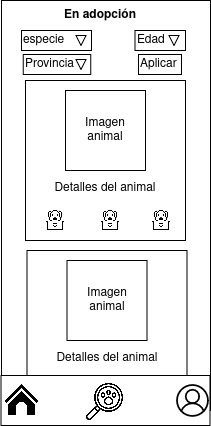
\includegraphics[width=0.31\linewidth]{"bocetos/iteracion 1/adopciones.drawio"}
	\caption{Boceto de visualización de animales en adopción}
	\label{fig:adopciones}
\end{figure}

Como podemos ver la idea para la página es mostrar una lista con los animales en busqueda de adopción en un contenedor con el siguiente formato:

\begin{itemize}
	\item \textbf{Imágenes de los animales}: Esto será un carrousel de imágenes en el que las asocaciones podrán mostrar el aspecto físico de sus animales.
	\item \textbf{Información específica}: Aquí se encontarán datos como el nombre, la raza y la edad del animal además de una descripción sobre el mismo.
	\item \textbf{Botones de acción}: las diferentes acciones a realizar serían la de solicituda de adopción, solicitud de acogida y apadrinamiento. Solicitud y apadrinamiento aparecerán solo si quiere la asocicación y este último tampoco aparecerá si ya está apadrinado.
\end{itemize}

\textbf{Implementación} %dimensiones móvil 506x901 \\

\begin{figure}[H]
		\centering
		\includegraphics[width=0.5\linewidth]{"Diseños finales/Iteracion 1/adopciones"}
		\caption{Vista final de la página que muestra a los animales en adopción en móviles}
		\label{fig:adopcionesDef}
\end{figure}


\begin{figure}[H]
	\centering
	\includegraphics[width=0.8\linewidth]{"Diseños finales/Iteracion 1/adopciones_web"}
	\caption{Vista final de la página que muestra a los animales en adopción en web}
	\label{fig:adopcionesDefWeb}
\end{figure}

Como podemos apreciar en ambos diseños se mantienen los componentes principales que mencionamos en los bocetos. Se ha usado el elemento de \textit{ion-card} para cada animal y en el se han añadido las imágenes pertinentes y una descripción del mismo.

A diferecia de la versión móvil, en web para que el espacio no esté totalmente vacío se ha decidido poner 2 tarjetas por fila, manteniendo su legibilidad y organización básica. \\

Para esta HU hemos tenido que crear las tablas en la base de datos de animales, usuarios de tipo asociación, pasíses y provincias, este último para poder hacer funcionar el filtro de localizaión para la búsqueda de adopciones. \\

En cuanto al servidor se han tenido que crear funciones para obtener a todos los animales o buscarlos en función de los filtros utilizados. \\

En la parte del cliente básicamente se ha creado la pantalla de vista de animales y un servicio el cual nos permite conectarnos al servidor para hacer las peticiones de obtención tanto de filtros como de las adopciones. \\ 



\Large{\textbf{HU.2 - Poner animales en adopción}}


En esta historia nos encargamos de de la subida de animales en adopción a la plataforma para que los distintos usuarios los puedan visualizar. \\

\textbf{Bocetos}

\begin{figure}[H]
	\centering
	\includegraphics[width=0.31\linewidth]{"bocetos/iteracion 1/poner-adopción.drawio"}
	\caption{Boceto de página para añadir animales en adopción}
	\label{fig:poner-adopcion}
\end{figure}

Podemos apreciar que en esta página será básicamente un formulario que se divide en 3 partes diferenciadas: \\ 

\begin{itemize}
	\item \textbf{Datos básicos}: Este apartado contendrá la información necesaria (nombre, edad, especie, etc.) del animal en cuestión.
	\item \textbf{Imágenes}: En este apartado se pondrán las fotos que se quiera.
	\item \textbf{Datos específicos}: Estos son un conjunto de \textit{checkboxes} en los que se dará informción mas detallada y clínica sobre tratamientos a los que haya sido sometidos como por ejemplo castración o desparasitación entre otros.
\end{itemize}

\textbf{Implementación} \\

\begin{figure}[H]
	\centering
	\includegraphics[width=0.7\linewidth]{"Diseños finales/Iteracion 1/subidaAdopciones"}
	\caption{ Diseño de subida de adopciones móvil}
	\label{fig:subidaadopciones}
\end{figure}


\begin{figure}[H]
	\centering
	\includegraphics[width=0.7\linewidth]{"Diseños finales/Iteracion 1/subAdopWeb"}
	\caption{Diseño de subida de adopciones web}
	\label{fig:subadopweb}
\end{figure}

Como podemos apreciar en diferencia con el boceto los campos básicos aparecen en vértical de uno en uno en lugar de ir por bloques, esto se ha decido para aportar mayor legibilidad y orden, ya que de la otra manera tendrían tamaños irregulares y en ciertos modelos de teléfono probablemnete hubiese errores de superposción de elementos. \\

Para esta historia de usuario se ha modificado la tabla de animales para añadir los campos del checkbox y su correspondiente actualización en el backend. También hemos creado sendos métodos para la subida de imágenes, que se guardan en la carpeta uploads del servidor y se enlaza con una tupla en la tabla \textit{images} en la base de datos la cual contiene su nombre, y animales. En caso de que no se puedan añadir las imágenes se borrará de la base de datos al animal y se le avisará al usuario de que ha habido un error. \\


En cuanto al frontend hemos creado una página nueva en el proyecto la cual contiene un formulario y hemos hecho uso de FormGrup de Angular el cual nos permite hacer validaciones básicas como por ejemplo que una cadena tenga x caracteres, también se ha creado una función de validación de campos en la que se le da información al usuario de los errores mediante un elemento \textit{Toast}. \\

Por último se han creado también funciones para la obtención de imágenes que puede ser tanto desde la galería como desde la cámara en su versión móvil y solo desde los archivos en la versión web y la posibilidad de eliminar imágenes en caso de que no las queramos antes de la subida de los animales.\\

\Large{\textbf{Fin del Sprint}}

\textbf{Velocidad del Sprint} \\ \\
	Como bien se puede ver en la tabla del sprint 0 se habían planificado una serie de tareas para este mismo, pero una vez terminado debemos hacer una reestimación de la velocidad ya que el aprendizaje e investigación de las tecnologías ha suspuesto más tiempo del esperado, produciendo así retrasos en la realización de las tareas. Debido a esto la planificación estimada de los siguientes sprints quedaría de la siguiente manera: \\
	
	Sprint 2 \\
	\begin{figure}[H]
		\centering
		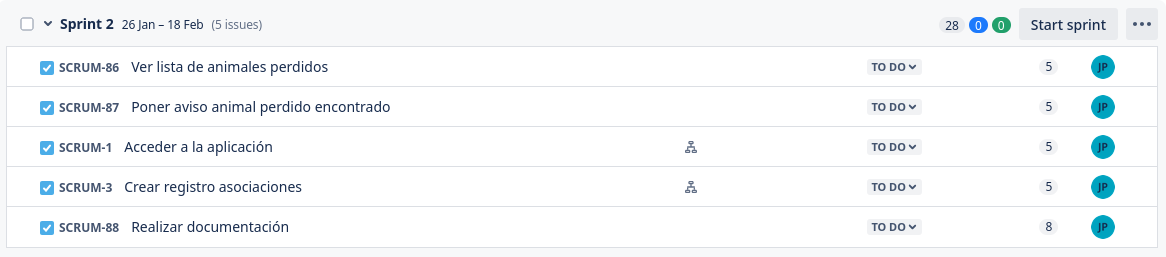
\includegraphics[width=1\linewidth]{newSprint2}
		\caption{Nuevas tareas sprint 2}
		\label{fig:newsprint2}
	\end{figure}
	
	
	Sprint 3 \\
	\begin{figure}[H]
		\centering
		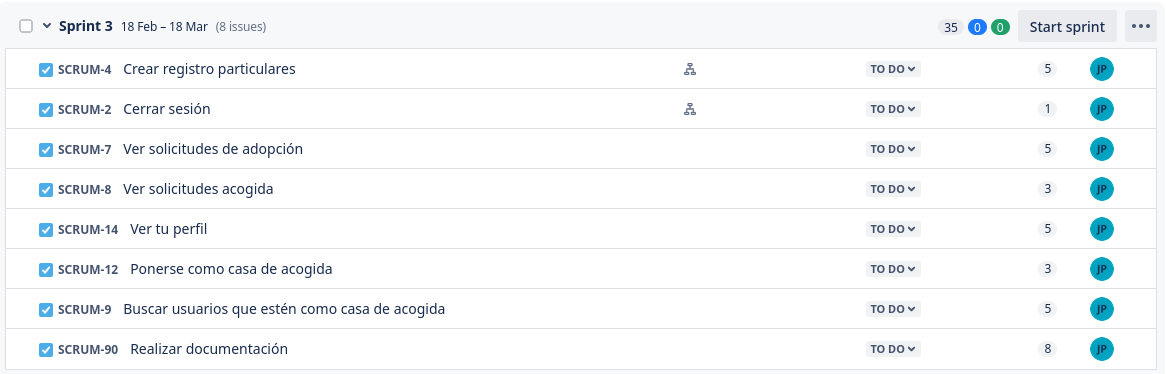
\includegraphics[width=1\linewidth]{newSprint3}
		\caption{Nuevas tareas sprint 3}
		\label{fig:newsprint3}
	\end{figure}
	
	Sprint 4 \\
	\begin{figure}[H]
		\centering
		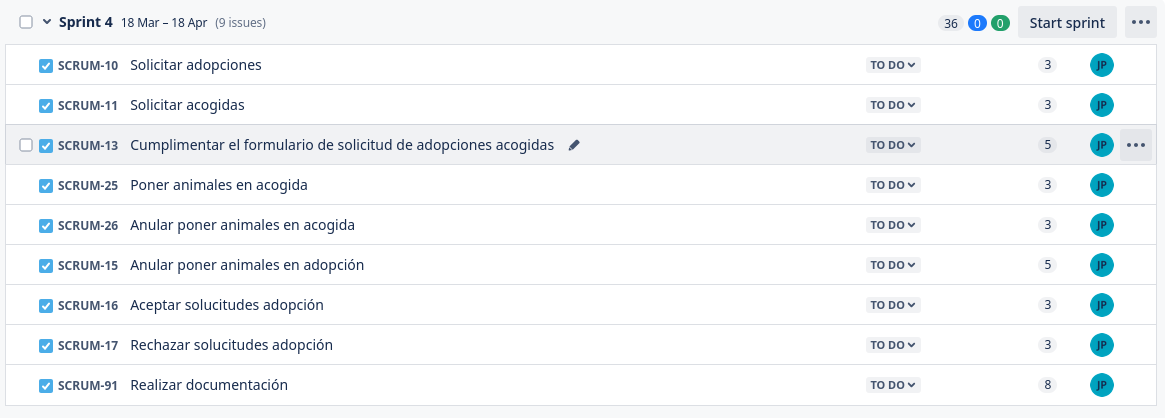
\includegraphics[width=1\linewidth]{newSprint4}
		\caption{Nuevas tareas sprint 4}
		\label{fig:newsprint4}
	\end{figure}
	
	
	Sprint 5 \\ 
	\begin{figure}[H]
		\centering
		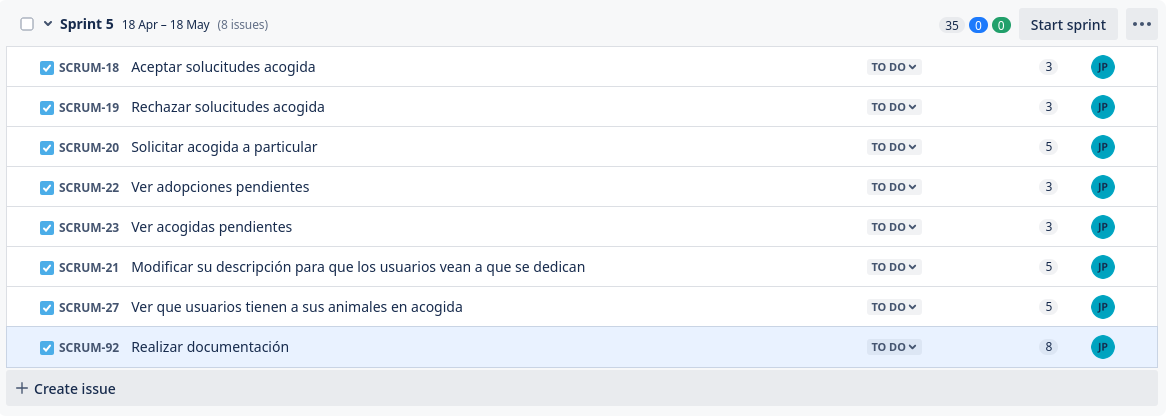
\includegraphics[width=1\linewidth]{newSprint5}
		\caption{Nuevas tareas sprint 5}
		\label{fig:newsprint5}
	\end{figure}
	
	El resto de tareas se moverán al backlog para su futura realización. \\ 
	
	\textbf{Backend} \\
	
	Como hemos visto en apartados anteriores (explicar en descripción de la propuesta que uso modelo-vista-controlador) en el back se encuentran tanto los controladores como los modelos para el acceso a la base de datos y su envío a la aplicación móvil. \\
	
	En la finalización del primer sprint la estructura de directorios es la siguiente:
	
	\begin{figure}[H]
		\centering
		\includegraphics[width=0.7\linewidth]{"sprint 1/directoriosBack"}
		\caption{Estructura de directorios del backend al final del sprint 1}
		\label{fig:directoriosback1}
	\end{figure}
	
	Además al utilizar un ORM se accede a la base de datos mediante clases por lo que para ilustrar su estructura se ha realizado un diagrama con sus relaciones y funciones básicas:
	
	\begin{figure}[H]
		\centering
		\includegraphics[width=1\linewidth]{"sprint 1/clases"}
		\caption{Diagrama de clases de la primera iteración}
		\label{fig:clases}
	\end{figure}


\subsection{Iteración 2}
\large{\textbf{Especificación de tareas}} \\

\begin{tabular}{|c|p{9.5cm}|p{1cm}|}
	\hline
	\multicolumn{3}{|c|}{\textbf{HU.3 - Ver lista de animales perdidos}} \\
	\hline
	\textbf{Id} & \textbf{Título de la tarea de desarrollo} & \textbf{Est. (días)} \\
	\hline
	3.1 & Realizar bocetos & 0.5 \\ \hline
	3.2 &  Implentar la lógica de acceso a los animales perdidos & 2 \\ \hline
	3.3 &  Implementar la interfaz para subir el aviso & 1 \\ \hline
	\multicolumn{3}{|c|}{\textbf{Pruebas de aceptación}} \\ \hline
	1 & \multicolumn{2}{|l|}{Mostrar mensaje en caso de que no haya animales perdidos} \\ \hline
	2 & \multicolumn{2}{|l|}{Mostrar lista de todos los animales perdidos} \\ \hline
	3 & \multicolumn{2}{|l|}{Que los filtros funcionen correctamente} \\ \hline
\end{tabular} \\ \\


\begin{tabular}{|c|p{9.5cm}|p{1cm}|}
	\hline
	\multicolumn{3}{|c|}{\textbf{HU.4 - Poner aviso de animal perdido encontrado}} \\
	\hline
	\textbf{Id} & \textbf{Título de la tarea de desarrollo} & \textbf{Est. (días)} \\
	\hline
	4.1 & Realizar bocetos & 0.5 \\ \hline
	4.2 &  Actualizar la logíca para añadir avisos a la base de datos & 2 \\ \hline
	4.3 &  Implementar la interfaz para subir el aviso & 1 \\ \hline
	\multicolumn{3}{|c|}{\textbf{Pruebas de aceptación}} \\ \hline
	1 & \multicolumn{2}{|p{10cm}|}{Comprobar que los campos deben estar cumplimentados antes de realizar la petición} \\ \hline
	2 & \multicolumn{2}{|p{10cm}|}{Que la imagen recortada se almacena apropiadamente} \\ \hline
	3 & \multicolumn{2}{|p{10cm}|}{Que la cámara funcione correctamente en dispositivos móviles} \\ \hline
\end{tabular} \\ \\

\begin{tabular}{|c|p{9.5cm}|p{1cm}|}
	\hline
	\multicolumn{3}{|c|}{\textbf{HU.5 - Crear registro de particulares}} \\
	\hline
	\textbf{Id} & \textbf{Título de la tarea de desarrollo} & \textbf{Est. (días} \\
	\hline
	5.1 & Realizar bocetos & 0.5 \\ \hline
	5.2 &  Implementar la lógica de registro & 2 \\ \hline
	5.3 &  Implementar la interfaz de registro & 1 \\ \hline
	\multicolumn{3}{|c|}{\textbf{Pruebas de aceptación}} \\ \hline
	1 & \multicolumn{2}{|p{10cm}|}{Comprobar que los campos deben estar cumplimentados correctamente antes de realizar la petición} \\ \hline
	2 & \multicolumn{2}{|p{10cm}|}{Asegurarse de que la imagen recortada se almacena apropiadamente} \\ \hline
	3 & \multicolumn{2}{|p{10cm}|}{Ver que la cámara funcione correctamente en dispositivos móviles} \\ \hline
	4 & \multicolumn{2}{|p{10cm}|}{Ver que los campos de ubicación se autocompletan correctamente} \\ \hline
\end{tabular} \\ \\\\

\begin{tabular}{|c|p{9.5cm}|p{1cm}|}
	\hline
	\multicolumn{3}{|c|}{\textbf{HU.6 - Acceder a la aplicación}} \\
	\hline
	\textbf{Id} & \textbf{Título de la tarea de desarrollo} & \textbf{Est. (días)} \\
	\hline
	6.1 &  Implementar la lógica asociada al inicio de sesión & 2 \\ \hline
	6.2 &  Implementar la interacción asociada al inicio de sesión de los asociaciones y particulares. & 1,5 \\ \hline
	6.3 &  Realizar bocetos. & 0.5 \\ \hline
\end{tabular} \\ \\




\begin{tabular}{|c|p{9.5cm}|p{1cm}|}
	\hline
	\multicolumn{3}{|c|}{\textbf{HU.7 - Cerrar sesión}} \\
	\hline
	\textbf{Id} & \textbf{Título de la tarea de desarrollo} & \textbf{Est. (días)} \\
	\hline
	7.1 & Realizar de bocetos & 0.5 \\ \hline
	7.2 &  Implementar la lógica asociada al cierre de sesión. & 1 \\ \hline
	7.3 &  Implementar interfaz asociada al cierre de sesión. & 0.5 \\ \hline
\end{tabular} \\ \\

\begin{tabular}{|c|p{9.5cm}|p{1cm}|}
	\hline
	\multicolumn{3}{|c|}{\textbf{HUT.1 - Realizar documentación}} \\
	\hline
	\textbf{Id} & \textbf{Título de la tarea de desarrollo} & \textbf{Est. (días)} \\
	\hline
	1.1 & Realizar documentación para cada tarea & 3 \\ \hline
	1.2 &  Añadir tareas a las historias de usuario & 0.5 \\ \hline
\end{tabular} \\ \\

\Large{\textbf{HU.3 - Ver lista de animales perdidos}} \\

En esta historia nos encargamos de la visualización de las publicaciones sobre animales perdidos que hayan subido los distintos usuarios filtrando como en la HU.1~\pageref{sec:hu1} por diversos filtros para hacer más eficiente la búsqueda.

\textbf{Bocetos}

\begin{figure}[h]
	\centering
	\includegraphics[width=0.31\linewidth]{"sprint 2/hu3/listaPerdidos"}
	\caption{Boceto de la página que lista los animales perdidos}
	\label{fig:listaperdidos}
\end{figure}

Como podemos ver la estructura es la misma que vimos en la página de lista de adopciones, ésta genera una cohesión en el diseño de la aplicación, haciéndola más intuitiva para el usuario final.

La única diferencia es que en este caso solo hay un único botón de acción que nos llevará a un chat con la persona que ha publicado el anuncio para poder obtener más información o para dar información sobre la perdida de la mascota.

\textbf{Implementación}
\begin{figure}[H]
	\centering
	\includegraphics[width=0.5\linewidth]{"sprint 2/hu3/disenoFinal"}
	\caption{Vista final de la página que muestra la lista de animales perdidos en móviles}
	\label{fig:listaAdop}
\end{figure}

\begin{figure}[H]
	\centering
	\includegraphics[width=0.8\linewidth]{"sprint 2/hu3/disenoFinalWeb"}
	\caption{Vista final de la página que lista a los animales perdidos en web}
	\label{fig:disenofinalweb}
\end{figure}

Como podemos apreciar no hay una gran diferencia entre el boceto y la implementación final en la aplicación ya que se mantien los elementos principales además se le ha añadido un botón en la esquina inferior izquierda que nos lleva a la página de para añadir una publicación de mascota perdida, la cual veremos más adelante.\\

En cuanto a la parte del servidor hemos tenido que crear dos tablas nuevas, una para los anuncios y otra para las imágenes de las mismas.\\

Además también se han creado funciones para el acceso a dichas tablas para su correcto tratamiento y envío a la aplicación móvil para que se muestren correctamente en el formato deseado. Para los filtros se ha reutilizado la mayor parte del código de la HU.1 por lo que eso ha permitido hacer más rápido el desarrollo de esta historia.\\ \\

\Large{\textbf{HU.4 - Poner aviso de animal perdido encontrado}}

En esta historia nos vamos a encargar de las tareas relacionadas con el añadido de posts a la sección de mascotas perdidas, para ello deberán rellenar un formulario con distinta información del animal. \\
\textbf{Bocetos}
\begin{figure}[H]
	\centering
	\includegraphics[width=0.31\linewidth]{"sprint 2/hu4/postearPerdido"}
	\caption{Boceto de la página para añadir publicaciones de animales perdidos}
	\label{fig:postearperdido}
\end{figure}

Como podemos ver a diferencia de la página en la que las asociaciones pueden añadir animales a su perfil en esta tenemos información diferente:

\begin{itemize}
	\item \textbf{Tipo de publicación}: Para este apartado tenemos 2 opciones puede que hayamos encontrado un animal en la calle y lo publiquemos en la aplicación para buscar a su dueño (Encontrado) o por el contrario, hemos perdido a nuestra mascota y queremos encontrarla, en este caso sería una publicación del tipo perdido. \\ 
	
	\item \textbf{Campos de ubicación}: Éstos los usaremos para el lugar en el que lo hemos perdido o encontrado al animal en cuestión, además ayudarán a la posterior búsqueda de los mismos gracias a la utilización de los filtros en la página de lista de animales perdidos. \\
	 
\end{itemize}

\textbf{Implementación}

\begin{figure}[H]
	\centering
	\includegraphics[width=0.8\linewidth]{"sprint 2/hu4/impPerdidos"}
	\caption{Vista final de la página para añadir animales perdidos en móviles}
	\label{fig:impperdidos}
\end{figure}

\begin{figure}[H]
	\centering
	\includegraphics[width=0.8\linewidth]{"sprint 2/hu4/impPerdidosWeb"}
	\caption{Vista final de la página para añadir animales perdidos en web}
	\label{fig:impperdidosweb}
\end{figure}

Como podemos ver en la implentación para móviles en función del tipo de publicación que sea la información que rellena el usuario es ligeramente diferente ya que por ejemplo alguien que haya encontrado un perro perdido no va a saber su nombre como si lo haría el dueño del animal. El otro campo es la zona de desaparición  para el caso de perder a tu mascota, que sería el lugar de de recogida para el que lo encuentre. \\

Además en esta historia cabe destacar de que se soluciona un problema existente en las imágenes, ahora todas deben tener el mismo ratio de escala, para así cuando se vizualicen todas las publicaciones tengan el mismo tamaño, haciendo del diseño algo más consistente.\\

En cuanto a la base de datos gracias a la historia anterior no debemos añadir ninguna tabla más. Por otra parte hemos creado un endpoint del tipo \textit{POST} para añadir publicaciones a la base de datos. \\

Tabién hemos creado una función para añadir la publicación y para agregar las imágenes hemos reutilizado la creada en la adición de animales en adopción, coun unos pequeños cambios, como cambiar la ruta de almacenaje de las imágenes. \\ 

En el frontend hemos añadido la biblioteca \textit{ngx-image-cropper} la cual nos permite recortar las imágenes con un ratio determinado como se ha mencionado anteriormente, lo que ha acelerado el desarrollo de la historia. El funcionamiento es sencillo, cada vez que subimos una imágen se nos pedirá que la recortemos con la proporción adecuada pudiendo mover el selector por la image y haciendola más grande o más pequeña en función de nuestras necesidades. \\


\Large{\textbf{HU.5 - Crear registro de particulares}}

Esta historia, como su título nos indica comprende la creación del registro de usuarios, esta página se trata de un formulario con la información pertinente para su correcta gestión.\\

\textbf{Bocetos}
\begin{figure}[H]
	\centering
	\includegraphics[width=0.31\linewidth]{"sprint 2/hu5/registro_particulares"}
	\caption{Boceto de la página de registro de particulares}
	\label{fig:registroparticulares}
\end{figure}

La estructura básica de la página es simple, tenemos un conjunto de campos a cubrir y un botón el cual nos permitirá envíar la información al servidor para realizar la creación del mismo. \\

\textbf{Implementación}

\begin{figure}[H]
	\centering
	\includegraphics[width=0.7\linewidth]{"sprint 2/hu5/impRegistroParticulares"}
	\caption{Vista final de la página de creación de particulares en móviles}
	\label{fig:impregistroparticulares}
\end{figure}

\begin{figure}[H]
	\centering
	\includegraphics[width=0.7\linewidth]{"sprint 2/hu5/impRegistroParticularesWeb"}
	\caption{Vista final de la página de creación de particulares en Web}
	\label{fig:impregistroparticularesweb}
\end{figure}


Como vemos en cuanto a diferencia con los bocetos no hay demasiada en la implementación final lo que sí que podemos observar es que a diferencia de los otros formularios en el tema claro de éste los elementos tienen un color de fondo grisaceo asemejándose así al tema oscuro. Esto se ha decidido para hacer más homogénea la aplicación. Cabe destacar que este cambio ha sido aplicado al resto de formularios de forma retroactiva.

Además en cuanto al apartado de diseño también se ha ajustado el ancho en la versión web, para que los elementos no ocupen todo el ancho de la página.

En cuanto a la programación, debemos destacar los siguientes aspectos:

\begin{itemize}
	\item \textbf{Obtención dinámica de localización}: Para esta historia se ha implementado la geolocalización, lo que nos permite acceder a la ubicación del dispositivo y así autocompletar la información referente a la ubicación sin que el usuario tenga que hacer nada. Para ello hemos hecho uso de la biblioteca \textit{opencage-api-client}, la cual nos devuelve información sobre la locacización actual del dispositivo, en este caso utilizamos la provincia y desde ella obtenemos el país al cual pertenece en nuestra base de datos. 
	
	En caso de no tener activada la geolocaclización el usuario debe introducirlo manualmente, si no la aplicación le avisará de un error.
	
	Esto se ha implementado también en la página de publicar animales perdidos por motivos de practicidad.
	

	\item \textbf{Control de errores}: En caso de que el usuario se deje alguno de los campos obligatorios sin rellenar cuando pulse el botón de crear cuenta se le avisará mediante un \textit{toast}, en este caso todos los campos son obligatorios a excepción de la fotografía.
	
	Además también en el momento de la inserción se comprueba previamente si tanto el correo como el nombre de usuario están en uso actualmente, y, en caso de estarlo, se le notificará al usuario que alguno de éstos ya está en uso.
\end{itemize}

En el servidor se han creado funciones para la obtención dinámica de la ubicación, para ello éste recibe la provincia y de ella obtiene el país al que pertenece y se retorna a la aplicación un estructura con todos los países y sus provincias la provincia actual y el país al que pertenece, esto es lo que en el front end nos permite rellenar los selectores correctamente.

Se ha creado un endpoint para la información que tenga que ver con los usuarios, en este caso su creación y la comprobación de que el usuario a registrar en la aplicación no exista actualmente.

Un detalle a comentar es que en el diagrama de la iteración 1 los usuarios no tenían el campo de contraseña, este ya se ha añadido como se reflejará en el diagrama al final de esta iteración. \\


\Large{\textbf{HU.6 - Acceder a la aplicación}} 

En el desarrollo de esta historia hemos realizado la creación de la página de \textit{log in} para que los distintos usuarios puedan acceder a la misma y acceder a contenido limitado o especíco de un tipo de usuario concreto. \\ 

\textbf{Bocetos}


\begin{figure}[H]
	\centering
	\includegraphics[width=0.31\linewidth]{"sprint 2/hu6/login"}
	\caption{Boceto de la pantalla de acceso}
	\label{fig:login}
\end{figure}

Como podemos apreciar en el boceto la página contará con un pequeño formulario de inicio de sesión en el cual se deberá rellenar con el nombre de usuario y su contraseña pertinente. Además también vemos que desde esta página se podrá ir a la de registro. \\

\textbf{Implementación}

\begin{figure}[H]
	\centering
	\includegraphics[width=0.7\linewidth]{"sprint 2/hu6/ImpLoginMovil"}
	\caption{Diseño final de la página de acceso en móviles}
	\label{fig:imploginmovil}
\end{figure}

\begin{figure}[H]
	\centering
	\includegraphics[width=0.7\linewidth]{"sprint 2/hu6/ImpLoginWeb"}
	\caption{Diseño final de la página de acceso en web}
	\label{fig:imploginweb}
\end{figure}

\textbf{Implentación} \\

Como podemos ver en el diseño final no ha habido cambios significativos con respecto a los bocetos, pero si que se ha cambiado la estética en los botones de la aplicación, esto se ha hecho con caracter retroactivo aplicándose al resto de páginas, esto se ha hecho para hacer una interfaz más acorde a las corrientes actuales.

En esta página hemos creado un pequeño formulario con los datos de inicio de sesión que se enviarán al servidor en cuanto le demos aceptar.

Si se hayan fallos en las credenciales se le notificará al usuario que ha habido un error, si son correctas se accederá de manera normal a la aplicación.

Para mantener al usuario conectado hemos hecho uso sesiones. Para esto hemos instalado la biblioteca \textit{express-session} la cual nos permite almacenar los datos que necesitemos para mantener las sesiones de los usuarios además de envíar una cookie con el id de la sessión al usuario, lo que nos permitirá acceder a su información cuando se hagan peticiones al servidor.

Hemos creado un endpoint para el login (/api/login) en el cual tenemos 2 métodos, uno para comprobar si las credenciales son correctas y otro para saber si el usuario tiene ya una sesión activa. En el primero debemos aseguranos de crear la sesión y enviarle la cookie a la aplicación.

Con todo esto ya tenemos terminada la lógica del acceso en el servidor, pero también hemos tenido que controlar el acceso a las páginas de la aplicación a las que no se puede acceder si no estás logueado y hacer que aparezcan o no ciertos elementos en función del tipo de usuario que esté conectado, esto además se irá actualizando co el tiempo a medida que se vayan creando nuevas páginas. \\

\Large{\textbf{Fin del sprint}} \\

La estructura actual de directorios en el backend es la siguiente: 

\begin{figure}[H]
	\centering
	\includegraphics[width=0.7\linewidth]{"sprint 2/directoriosBackS2"}
	\caption{Estructura de directorios del backend al final del sprint}
	\label{fig:directoriosbacks2}
\end{figure}

Además también se ha actualizado el diagrama de clases, aunque en esta iteración no se han creado nuevas clases se han realizado otros cambios, como añadir los métodos necesarios para la búsqueda de país a partir de una provincia o los asociados a la creación de usuarios.

\begin{figure}[H]
	\centering
	\includegraphics[width=1\linewidth]{"sprint 2/clases"}
	\caption{Diagrama de clases de la segunda iteración}
	\label{fig:clases2}
\end{figure}



















